% Section content template for individual Educative lessons
% This file contains the actual content for a specific section
% Generated from Educative API section content

% Section: Initial Design of Quora
% Section ID: 6337842040537088
% Section Slug: initial-design-of-quora
% Generated: 2025-12-07T22:55:40.197810

\subsection{Initial design}\label{0NRV7lQdz6TWCXSsUTKQ4}
\\
The initial design of Quora will be composed of the following building blocks and components:

\begin{itemize}
\item
\protect\phantomsection\label{M9gCENDNWDf7WcruAf-Po}
\textbf{Web and application servers}: A typical Quora page is generated by various services. The web and application servers maintain various processes to generate a webpage. The web servers have manager processes and the application servers have worker processes for handling various requests. The manager processes distribute work among the worker processes using a router library. The router library is enqueued with tasks by the manager processes and dequeued by worker processes. Each application server maintains several in-memory queues to handle different user requests. The following illustration provides an abstract view of web and application servers:
\end{itemize}

\begin{figure}[htbp]
 \centering
 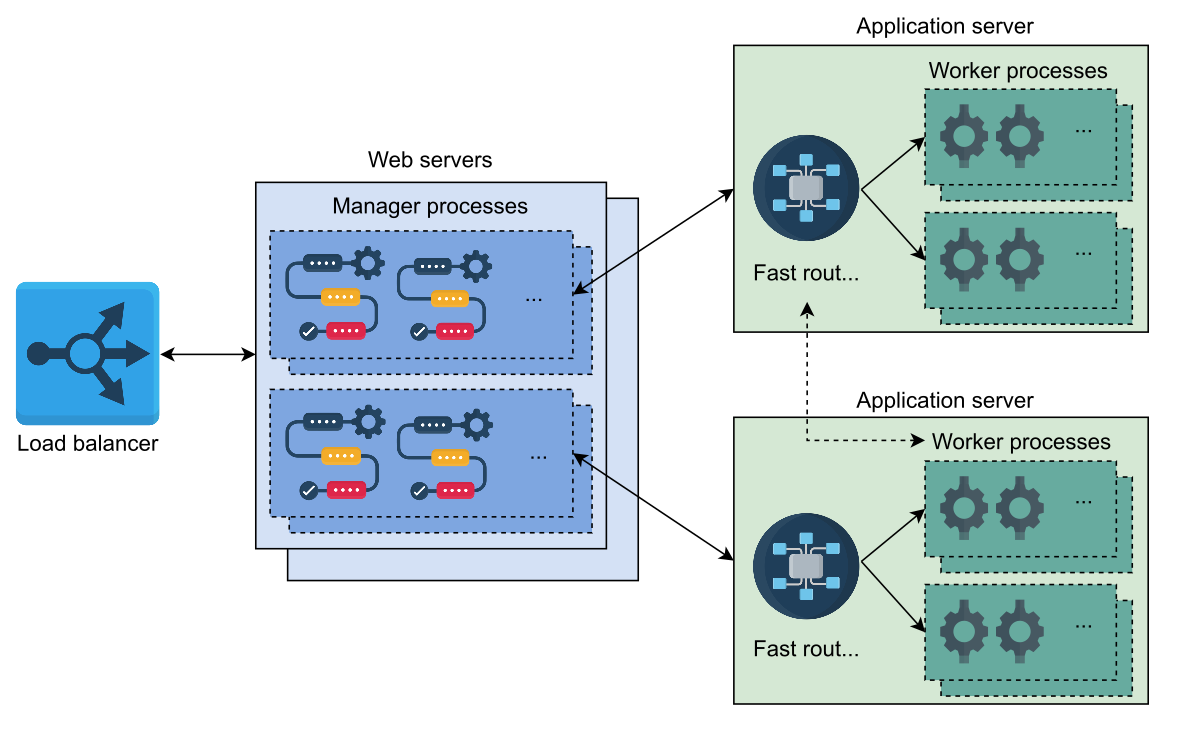
\includegraphics[width=0.5\textwidth]{Images/chapter_27/section_6337842040537088/6074511837626368.png}
 \caption{Web and application servers at Quora}
\end{figure}

\begin{itemize}
\item
\protect\phantomsection\label{isPHGuEFv4aWQ9Iz6pGH5}
\textbf{Data stores}: Different types of data require storage in different data stores. We can use critical data like questions, answers, comments, and upvotes/downvotes in a relational database like MySQL because it offers a higher degree of consistency. NoSQL databases like HBase can be used to store the number of views of a page, scores used to rank answers, and the extracted features from data to be used for recommendations later on. Because recomputing features is an expensive operation, HBase can be a good option to store and retrieve data at high bandwidth. We require high read/write throughput because big data processing systems use high parallelism to efficiently get the required statistics. Also, blob storage is required to store videos and images posted in questions and answers.
\end{itemize}

Quora was founded in 2009, whereas HBase was developed in 2008 by Apache. Because it is open-source and modeled after Google's BigTable, it is suitable for storing a large amount of small-sized data. Furthermore , it has high read/write throughput. Therefore, it was a natural choice for Quora to use in its inception.

\begin{itemize}
\item
\protect\phantomsection\label{soWfLC9Q-eE1o-xJO8Eld}
\textbf{Distributed cache}: For performance improvement, two distributed cache systems are used: Memcached and Redis. Memcached is primarily used to store frequently accessed critical data that is otherwise stored in MySQL. On the other hand, Redis is mainly used to store an online view counter of answers because it allows in-store increments. Therefore, two cache systems are employed according to their use case. Apart from these two, CDNs serve frequently accessed videos and images.
\item
\protect\phantomsection\label{tyoZsQAAP3AjR-GcE_UJL}
\textbf{Compute servers}: A set of compute servers are required to facilitate features like recommendations and ranking based on a set of attributes. These features can be computed in online(Recommendations are computed as soon as they are requested.) or offline(Recommendations are computed beforehand and served when requested.) mode. The compute servers use machine learning (ML) technology to provide effective recommendations. Naturally, these compute servers have a substantially high amount of RAM and processing power.
\end{itemize}
\\
Of course, other basic building blocks like load balancers, monitoring services, and rate limiters will also be part of the design. A high-level design is provided below:

\begin{figure}[htbp]
 \centering
 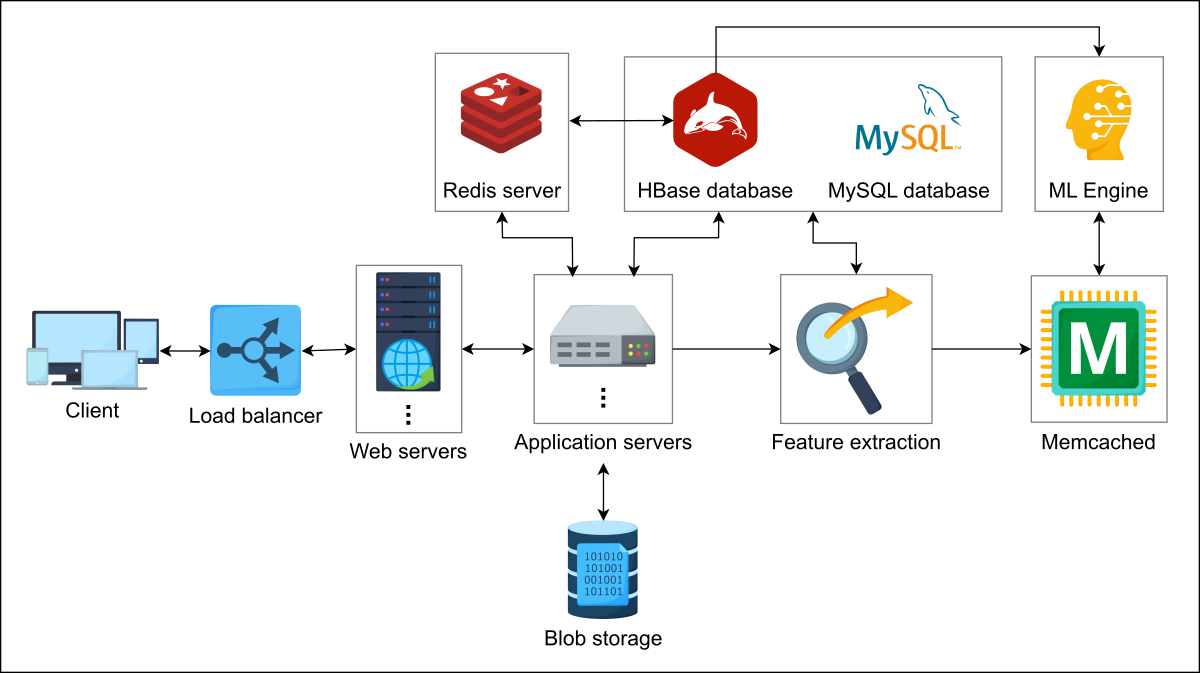
\includegraphics[width=0.5\textwidth]{Images/chapter_27/section_6337842040537088/5312892549595136.png}
 \caption{The high-level design of Quora}
\end{figure}

Why does Quora use both Memcached and Redis in its architecture? What are the strengths of each? Can you explain the specific advantages of using both systems?
\\
Use the AI assessment widget below to submit your solution and get an interactive response.

\textbf{Question:}

Why do we use two caching systems for Quora?

\textbf{Reference Answer:}

Quora's use of both Memcached and Redis is to leverage each system's strengths. Memcached is optimized for simple key-value storage and quick retrieval of frequently accessed MySQL data, making it perfect for caching static content like questions and answers. Redis , on the other hand, offers specialized features like atomic increments, which is crucial for Quora's real-time view counter functionality. Using a single caching solution would force compromises, either losing Memcached's simplicity and performance for static content or giving up Redis's advanced features for dynamic data operations.

\subsection{Workflow}\label{iszfbJb1NSBFXShMpacN-}
\\
The design of Quora is complex because we have a large number of functional and non-functional requirements. Therefore, we'll explain the workflow on the basis of each feature:

\begin{itemize}
\item
\protect\phantomsection\label{9mKsiTju3dJF8W_JYZ_Sn}
\textbf{Posting question, answers, comments}: The web servers receive user requests through the load balancer and direct them to the application servers. Meanwhile, the web servers generate part of the web page and let the worker process in the application servers do the rest of the page generation. The questions and answers data is stored in a MySQL database, whereas any videos and images are stored in the blob storage. A similar approach is used to post comments and upvote or downvote answers. Task prioritization is performed by employing different queues for different tasks. We perform prioritization because certain tasks require immediate attention---for example, fetching data from the database for a user request---while others are not so urgent---for example, sending a weekly email digest. The worker processes will perform tasks by fetching from these queues.
\end{itemize}

\begin{quote}
\textbf{Quiz:}
\textbf{Question 1:} When would a service like Quora require a notifications feature?
\textbf{Answer:} Quora will need a notification service in the following scenarios: - A

user posts a question on a topic subscribed by a would-be respondent. - A user posts an answer to a question asked by another user. - A post a user is interested in or wrote received new comments or upvotes/downvotes, and so on.
\textbf{Question 2:} How is it possible for Quora to send notifications to users through the above-described mechanism?
\textbf{Answer:} Since tasks are added to different priority queues, it is possible to maintain a queue for notifications. While higher priority tasks are enqueued to high-priority queues, a notification task will be added to a medium or lower priority queue. The illustration below visualizes the described concept.
\end{quote}

\begin{itemize}
\item
\protect\phantomsection\label{hT1eVPS7p--apFaf-eXF0}
\textbf{Answer ranking system}: Answers to questions can be sorted based on date. Although it is convenient to develop a ranking system on the basis of date (using time stamps), users prefer to see the most appropriate answer at the top. Therefore, Quora uses ML to rank answers. Different features are extracted over time and stored in the HBase for each type of question. These features are forwarded to the ML engine to rank the most useful answer at the top. We cannot use the number of upvotes as the only metric for ranking answers because a good number of answers can be jokes---and such answers also get a lot of upvotes. It is good to implement the ranking system offline because good answers get upvotes and views over time. Also, the offline mode poses a lesser burden on the infrastructure. Implementing the ranking system offline and the need for special ML hardware makes it suitable to use some public cloud elastic services.
\item
\protect\phantomsection\label{5mfeNSFDhA-vJDXLQPBz-}
\textbf{Recommendation system}: The recommendation system is responsible for several features. For example, we might need to develop a user feed, find related questions and ads, recommend questions to potential respondents, and even highlight duplicate content and content in violation of the service's terms of use. Unlike the answer ranking system, the recommendation system must provide both online(While the user requests the page, provide the recommendations during the API call) and offline(Perform the computations beforehand to prepare the recommendations and deliver when requested.) services. This system receives requests from the application server and forwards selected features to the ML engine.
\item
\protect\phantomsection\label{lE9z1JtsDjY_EmJziayy0}
\textbf{Search feature}: Over time, as questions and answers are fed to the Quora system, it is possible to build an index in the HBase. User search queries are matched against the index, and related content is suggested to the user. Frequently accessed indexes can be served from cache for low latency. The index can be constructed from questions, answers, topics labels, and usernames. Tokenization of the search index returns the same results for reordered words also (see \href{https://www.educative.io/courses/grokking-the-system-design-interview/scaling-search-and-indexing}{Scaling Search and Indexing} in \textbf{Distributed Search} chapter for more details).
\end{itemize}

\begin{itemize}
\tightlist
\item
Quora is mostly built on Amazon Web Services (AWS).
\item
Initially, Quora used Amazon's EC2 instances as their application servers used eight cores with an 8 MB cache.
\item
Quora used the search server called Sphinx. Later , because of its slow performance, Quora custom-built its search engine using Thrift and Python Unicode libraries only.
\item
The full-text search feature was launched by Quora in 2013. Before that, it was possible to get results for individual words only.
\end{itemize}

How does Quora use both HBase indexing and caching to optimize its search functionality? What specific roles do each play in balancing search accuracy and performance?
\\
Use the AI assessment widget below to submit your solution and get an interactive response.

\textbf{Question:}

What are the benefits of this dual approach?

\textbf{Reference Answer:}

Quora's search system combines HBase indexing and caching for efficiency. HBase indexes tokenized content from questions, answers, topics, and usernames, ensuring comprehensive searchability. The cache stores frequent queries, reducing latency and system load. Without caching, searches would be slower, and without indexing, the cache alone wouldn't be sufficient. This dual approach balances completeness and performance.

\subsection{API design}\label{-EIG-XU7OiH8au0G-o0H1}
\\
We'll design the API calls for Quora in this section. We'll define APIs for the following features only:

\begin{itemize}
\item
\protect\phantomsection\label{PKgKVCS0_Ls3dlx7q3U6a}
Post a question
\item
\protect\phantomsection\label{nKCh4DqGYsc8DRuHLZMb2}
Post an answer
\item
\protect\phantomsection\label{VXMPp2ofFKoANTUE6em95}
Upvote or downvote a question or answer
\item
\protect\phantomsection\label{kssHnnc_ZwA-I9rdOQySN}
Comment on an answer
\item
\protect\phantomsection\label{ZK38z2jRh3ed0lDWLB7Lr}
Search
\end{itemize}
\begin{quote}
\textbf{Note:} We don't consider APIs for a recommendation system or ranking because they are not placed as an explicit request by the user. Instead, the web server coordinates with other components to ensure the service.
\end{quote}
\subsubsection{Post a question}\label{4JEUUd9YqH9uvG74BbmIY}
\\
The POST method of HTTP is used to call the \texttt{/postQuestion} API:

\begin{lstlisting}[language=JavaScript]
postQuestion(user_id, question, description, topic_label, video, image)
\end{lstlisting}

Let's understand each parameter of the API call:

\begin{table}[htbp]
\centering
\small
\adjustbox{max width=\textwidth}{
\begin{tabular}{|p{0.208\textwidth}|p{0.742\textwidth}|}
\hline
\textbf{Parameter} & \textbf{Description} \\
\hline
\hline
\texttt{user\_id} & This is the unique identification of the user that posts the question. \\
\hline
\texttt{question} & This is the text of the question posed by the user. \\
\hline
\texttt{description} & This is the description of a question. This is an optional field. \\
\hline
\texttt{topic\_label} & This represents a list of domains to which the user's question is related. \\
\hline
\texttt{video} & This is a video file embedded in a user question. \\
\hline
\texttt{image} & This is an image that is a part of a user question. \\
\hline
\end{tabular}
}
\end{table}

The video and image parameters can be \texttt{NULL} if no image or video is embedded within the question. Otherwise , it is uploaded as part of the question.

\subsubsection{Post an answer}\label{9TkDhY3ElksVq9O_Ofgsd}
\\
For posting an answer, the POST method is a suitable choice for \texttt{/postAnswer} API:

\begin{lstlisting}[language=JavaScript]
postAnswer(user_id, question_id, answer_text, video, image)
\end{lstlisting}

\begin{table}[htbp]
\centering
\small
\adjustbox{max width=\textwidth}{
\begin{tabular}{|p{0.208\textwidth}|p{0.742\textwidth}|}
\hline
\textbf{Parameter} & \textbf{Description} \\
\hline
\hline
\texttt{question\_id} & This refers to the question the answer is posted against. \\
\hline
\texttt{answer\_text} & This is the textual answer posted by the responder. \\
\hline
\end{tabular}
}
\end{table}

The rest of the parameters are self-explanatory.

\subsubsection{Upvote an answer}\label{XwSm1IMEIbwDOMwOIKl9_}
\\
The \texttt{/upvote} API is below:

\begin{lstlisting}[language=JavaScript]
upvote(user_id, question_id, answer_id)
\end{lstlisting}

\begin{table}[htbp]
\centering
\small
\adjustbox{max width=\textwidth}{
\begin{tabular}{|p{0.208\textwidth}|p{0.742\textwidth}|}
\hline
\textbf{Parameter} & \textbf{Description} \\
\hline
\hline
\texttt{user\_id} & This represents the user upvoting the answer. \\
\hline
\texttt{answer\_id} & This represents the identity of the answer that is upvoted for a particular question, which is identified by the \texttt{question\_id}\emph{.} \\
\hline
\end{tabular}
}
\end{table}

\begin{quote}
\textbf{Note:} The downvote API is the same as the upvote API because both are similar functionalities.
\end{quote}
\subsubsection{Comment on an answer}\label{m1xnhGS0Yp3VA9Qsq2fMF}
\\
The \texttt{/comment} API has the following structure:

\begin{lstlisting}[language=JavaScript]
comment(user_id, answer_id, comment_text)
\end{lstlisting}

\begin{table}[htbp]
\centering
\small
\adjustbox{max width=\textwidth}{
\begin{tabular}{|p{0.208\textwidth}|p{0.742\textwidth}|}
\hline
\textbf{Parameter} & \textbf{Description} \\
\hline
\hline
\texttt{user\_id} & It represents the user commenting on the answer. \\
\hline
\texttt{comment\_text} & It represents the text a user posts against an answer identified by the \texttt{answer\_id}. \\
\hline
\end{tabular}
}
\end{table}

\subsubsection{Search}\label{2WJ6dR0cdcommGW3hGz6M}
\\
The \texttt{/search} API has the following details:

\begin{lstlisting}[language=JavaScript]
search(user_id, search_text)
\end{lstlisting}

\begin{table}[htbp]
\centering
\small
\adjustbox{max width=\textwidth}{
\begin{tabular}{|p{0.208\textwidth}|p{0.742\textwidth}|}
\hline
\textbf{Parameter} & \textbf{Description} \\
\hline
\hline
\texttt{user\_id} & This is the \texttt{user\_id} performing the search query. It is optional in this case because a non-registered user can also search for questions. \\
\hline
\texttt{search\_text} & This is the search query entered by a user. \\
\hline
\end{tabular}
}
\end{table}

\begin{quote}
We use a \href{https://www.educative.io/courses/grokking-the-system-design-interview/system-design-sequencer}{sequencer} to generate the different IDs mentioned in the API calls.
\end{quote}

\begin{quote}
\textbf{Quiz:}
\textbf{Question 1:} Why is there a custom routing layer between the web and application servers instead of a load-balancing layer?
\textbf{Answer:} The primary reason is performance. A generic load-balancing layer will have little application understandability and higher latency. As stated,

the manager processes generate the skeleton of the web page and leave the majority of the work to worker processes. In that sense, one manager process can generate multiple worker tasks. The custom  router library: Quora refers to it as ``Fastrouter''--it is a custom C++ built queue server.  is a queue between manager and worker, where any worker process can consume a task generated by the manager process. This design improves the overall performance and supports scalability.
\end{quote}



% End of section content